\documentclass{article}

\textwidth=6.5in
\textheight=8.5in
\voffset=-54pt
\oddsidemargin=0in
\evensidemargin=0in
\setlength{\parskip}{8pt}
\setlength{\parindent}{0pt}

\usepackage{amsmath, amssymb}
\usepackage{ifthen}

\usepackage[inline]{enumitem}
\setlist{topsep=0pt, parsep=8pt}

\usepackage[rgb,table]{xcolor}\convertcolorsUfalse
\usepackage{graphicx}

% change hyperref options
\PassOptionsToPackage{hyphens}{url}
\usepackage[bookmarks,colorlinks,linkcolor=black,citecolor=blue,pdfstartview=FitH,urlcolor=blue]{hyperref}
\hypersetup{pdfpagemode=UseNone}
\usepackage{bookmark}

\usepackage{graphicx}
\usepackage{multicol}
\usepackage{framed}
\usepackage{array}

\usepackage{icomma}

\usepackage{pifont}
\newenvironment{noanswer}{}{}

\usepackage{soul}

\usepackage{pgfplots}
\pgfplotsset{compat=1.18}  
\pgfplotscreateplotcyclelist{mycolor}{black, blue, red, green!70!black, magenta, purple, cyan, orange }  
\pgfplotsset{
  disabledatascaling,
  cycle list=tikzcolor, 
  axis lines=middle,
  every axis plot/.style={no marks, thick},
  every axis/.style={
    enlarge x limits=false,
    enlarge y limits=auto,
    xlabel style={at={(current axis.right of origin)},anchor=west},
    ylabel style={at={(current axis.above origin)},anchor=south},
    % extra x and y ticks for asymptotes
    extra x tick style={grid=major, grid style={dashed,black}},
    extra y tick style={grid=major, grid style={dashed,black}},
    /pgf/number format/1000 sep={},
  },    
  tick label style = {font=\footnotesize, fill=\currentbgcolor, inner sep=0pt},    
  xticklabel shift=1pt,    
  scaled ticks=false,
  scaled y ticks=false,
  unbounded coords=jump,
  samples=101,
  minor tick length=0,
  scatter/classes={
    open={mark=*,draw=black,fill=white, mark size=2, thin},
    closed={mark=*,draw=black,fill=black, mark size=2, thin}
  },
  width=3in,
}
\pgfplotsset{open/.style={only marks, mark=*, fill=white, thin, mark size=2}}
\pgfplotsset{closed/.style={only marks, mark=*, draw=black, fill=black,
    thin, mark size=2}}
\pgfplotsset{labeled/.style={nodes near coords, only marks, mark=*, draw=black, fill=black, thin, mark size=2, point meta=explicit symbolic}}

\usepackage{tikz}
\usetikzlibrary{
  matrix,%
  % enables the snake paths
  decorations.pathmorphing,%
  % enables bigger arrows
  decorations.markings,%
  decorations.pathreplacing,%
  decorations.text,%
  calc,%
  patterns,%
  shapes.geometric,%
  arrows,
  decorations.shapes,
  positioning,
  plotmarks,
  intersections
}
\tikzset{>=latex} % sets default arrow type in tikz
\tikzset{font=\normalsize}
\tikzset{mark size=1.5pt, mark options=thin}
\tikzset{pin distance=4pt,
  every pin edge/.style={<-, thin, shorten <= -2pt}}

\interfootnotelinepenalty=10000
\renewcommand{\thefootnote}{(\arabic{footnote})}

\usepackage{multirow, bigdelim}

% change to \usepackage[sols]{handout} to see solutions
\usepackage{handout}

\newcommand\iscurrentenumi[1]{%
  \ifthenelse{\equal{#1}{\theenumi}}{}{#1}}
\setenumerate[1]{ref=\#\arabic*}
\setenumerate[2]{ref=\protect\iscurrentenumi{\theenumi}(\alph*)}
\newcommand\enumiiprefix[2]{%
  \ifthenelse{{\equal{#1}{\theenumi}}\AND{\equal{#2}{(\alph{enumii})}}}{}{}%
  \ifthenelse{{\equal{#1}{\theenumi}}\AND{\NOT{\equal{#2}{(\alph{enumii})}}}}{#2}{}%
  \ifthenelse{\equal{#1}{\theenumi}}{}{#1#2}%
}
\setenumerate[3]{ref=\protect\enumiiprefix{\theenumi}{(\alph{enumii})}\roman*}

\makeatletter

\newdimen\SOUL@dimen %new
\def\SOUL@ulunderline#1{{%
    \setbox\z@\hbox{#1}%
    % \dimen@=\wd\z@
    \SOUL@dimen=\wd\z@ %new
    \dimen@i=\SOUL@uloverlap
    \advance\SOUL@dimen2\dimen@i %\dimen@ exchanged too
    \rlap{%
      \null
      \kern-\dimen@i
      % \SOUL@ulcolor{\SOUL@ulleaders\hskip\dimen@}%
      \SOUL@ulcolor{\SOUL@ulleaders\hskip\SOUL@dimen}% new
    }%
    \unhcopy\z@
  }}

\makeatother

\renewcommand{\answer}[1]{#1}

\definecolor{purple}{rgb}{0.5,0,1.0}
\definecolor{hotpink}{rgb}{1, 0, 0.5}

\definecolor{skyblue}{rgb}{0, 0.5, 1}

\newcommand{\highlight}[1]{\boldmath\hl{\textbf{#1}}\unboldmath}

\newcommand{\goal}[1]{\textbf{\textcolor{skyblue}{#1}}}

\usepackage{amsthm}

% make URLs print in the same font
\usepackage{url}
\urlstyle{same}

\usepackage{pifont}
\def\exend{\hfill\ding{118}}

%\makeatletter\@addtoreset{equation}{section}\makeatother
%\renewcommand{\theequation}{\arabic{section}.\arabic{equation}}

\newtheoremstyle{theorem}% name
{8pt}%      Space above
{0pt}%      Space below
{\itshape}%         Body font
{}%         Indent amount (empty = no indent, \parindent = para indent)
{\bfseries}% Thm head font
{.}%        Punctuation after thm head
{.5em}%     Space after thm head: " " = normal interword space;
                                %       \newline = linebreak
{}%         Thm head spec (can be left empty, meaning `normal')

\theoremstyle{theorem}

\let\Theorem\undefined
\newtheorem{Theorem}[equation]{Theorem}
\let\Definition\undefined
\newtheorem{Definition}[equation]{Definition}
\let\Summary\undefined
\newtheorem{Summary}[equation]{Summary}
\let\Conjecture\undefined
\newtheorem{Conjecture}[equation]{Conjecture}
\let\Fact\undefined
\newtheorem{Fact}[equation]{Fact}

\renewcommand{\thesubsection}{\arabic{subsection}}
\makeatletter
\def\@seccntformat#1{\@ifundefined{#1@cntformat}%
   {\csname the#1\endcsname\quad}%       default
   {\csname #1@cntformat\endcsname}}%    enable individual control
\newcommand\section@cntformat{}
\makeatother

  \usepackage{exam}

\usepackage{fancyhdr}
\lhead{\textcolor{white}{This content is protected and may not be shared, uploaded, or distributed.}}
\rhead{}
\rfoot{\vspace*{\fill}\footnotesize\textcopyright{} \emph{Harvard Math Ma}}
\renewcommand{\headrulewidth}{0pt}
\pagestyle{fancy}
\begin{document}

  \title{Final Exam Practice 3}

\instructions{instructions.tex}{}

\listofproblems

\begin{enumerate}

\item \label{fall2018-midterm-7-shortened} \points{13} 

  Kate has designed a new productivity app that is for sale in the app store. Based on extensive marketing research, she notices the number of downloads per day depends on how she prices it. Here is what she observes:
  \begin{itemize}
  \item If she prices the app anywhere from \$0 to \$5, there are 1000 downloads per day.
  \item If she prices the app between \$5 and \$7, people interpret the higher price as a sign of quality, and there are 10 additional downloads per day for each 10 cent increase in price. 
  \item If she prices the app at more than \$7, people start to think the app is overpriced, so there are 30 fewer downloads per day for every 10 cent increase in price.
  \end{itemize}
  Let $D(p)$ be the number of downloads per day if the app is priced at $p$ cents.

  \begin{enumerate}        

  \item
    \begin{problem}[\vfill]
      Sketch a graph of $D(p)$. 
    \end{problem}

    \begin{solution}
      The graph is constant on $[0, 500]$. On $(500, 700)$, it has a slope of 10 downloads per day per 10 cents, or 1 download per day per cent. When $p > 700$, $D(p)$ has a slope of $-30$ downloads per day per 10 cents, or $-3$ downloads per day per cent.
      \begin{center}
        \answer{
          \begin{tikzpicture}
            \begin{axis}[axis equal image, ymin=0, xtick={500, 700}, xlabel={price (cents)}, ylabel={downloads per day}, enlarge x limits=auto, ytick={1000}]
              \addplot+[sharp plot] coordinates { (0, 1000) (500, 1000) (700, 1200) (1100, 0)}; 
            \end{axis}
          \end{tikzpicture}
        }
      \end{center}
    \end{solution}    

  \item
    \begin{problem}[\vfill\newpage]
      Write a formula for $D(p)$. 
    \end{problem}

    \begin{solution}
      On $[0, 500]$, we know $D(p) = 1000$.

      The second piece of the graph has slope 1 and includes the point $(500, 1000)$. So, the equation of this piece is $D - 1000 = 1 (p - 500)$, or $D = p + 500$.

      The third piece of the graph has slope $-3$ and includes the right endpoint of the second piece. Since the equation of the second piece is $D = p + 500$, its right endpoint is $(700, 1200)$. So, the equation of the third piece is $D - 1200 = -3(p - 700)$, or $D = -3(p - 700) + 1200 = -3p + 3300$. From this formula, we can see that $D = 0$ when $p = 1100$. It doesn't make sense to have negative downloads, so we should restrict the domain of $D(p)$ to $0 \leq p \leq 1100$.

      Thus, our formula is
      \[ 
        \boxed{D(p)=
          \begin{cases}
            1000 &\text{if } 0\leq p \leq 500 \\
            p+500 &\text{if } 500<p\leq 700 \\
            -3p+3300 &\text{if } 700<p\leq 1100
          \end{cases}}\]
    \end{solution}

  \item
    \begin{problem}[\stretch{0.5}]
      At what price does this model predict that Kate will receive 0 downloads per day?
    \end{problem}

    \begin{solution}
      We found already that this happens when $p = 1100$, or \fbox{\$11}.
    \end{solution}

  \item
    \begin{problem}[\vfill\newpage]
      Sketch the graph of $D'(p)$. Please indicate the units of each axis, and label any significant values. 
    \end{problem}

    \begin{solution}
      Since $D'(p)$ represents slope on the graph of $D(p)$, its units are $\dfrac{\text{downloads per day}}{\text{cent}}$, or downloads per day per cent.

      $D'(p)$ is undefined at $p = 500$ and $p = 700$ because the graph of $D(p)$ has corners there. We've already seen that the graph of $D(p)$ has slope 0 on $(0, 500)$, slope 1 on $(500, 700)$, and slope $-3$ on $(700, 1100)$.

      Since $D$ is undefined when $p < 0$ and when $p > 1100$, both $D'(0)$ and $D'(1100)$ are undefined. For example, think about the limit definition of $D'(1100)$: it's $\displaystyle \lim_{h \to 0} \frac{D(1100 + h) - D(1100)}{h}$. But when $h > 0$, the expression $\dfrac{D(1100 + h) - D(1100)}{h}$ is undefined, so $\displaystyle \lim_{h \to 0^+} \frac{D(1100 + h) - D(1100)}{h}$ is also undefined.

      So, the graph of $D'$ looks like this:
      \begin{center}
        \answer{
          \begin{tikzpicture}
            \begin{axis}[xtick={500, 700, 1100}, xlabel={price (cents)}, ylabel={downloads per day per cent}, enlarge x limits=auto, ytick={1, -3}, height=2in]
              \addplot+[domain=0:500, very thick] {0};%
              \addplot+[domain=500:700, very thick] {1};%
              \addplot+[domain=700:1100, very thick] {-3};%
              \addplot+[open] coordinates {(0, 0) (500, 0) (500, 1) (700, 1) (700, -3) (1100, -3)};% 
            \end{axis}
          \end{tikzpicture}
        }
      \end{center}
    \end{solution}

  \end{enumerate}

\item \label{fall2012-ma-midterm1-3-II} \points{8} 

  Suppose $g(x)$ is an unknown function; all we know about it is:
  \begin{itemize}[nosep]
  \item It has domain $[-6, 6]$.
  \item It's continuous on $(-4, 4)$.
  \item Its graph passes through the points $(-5, 1)$, $(-3, 4)$, $(1, -3)$, and $(5, 2)$.
  \end{itemize}
  \begin{center}
    \begin{tikzpicture}
      \begin{axis}[title={Known points on the graph of $g(x)$}, xtick={-6, ..., 6}, ytick={-3, ..., 4}, xmin=-6, xmax=6, enlarge x limits=auto]
        \addplot+[closed] coordinates { (-5, 1) (-3, 4) (1, -3) (5, 2) };
      \end{axis}
    \end{tikzpicture}
  \end{center}

  Decide whether each statement below is definitely true. If so, briefly explain why. If not, sketch a possible $g(x)$ (satisfying the description above) for which the statement is false.

  \begin{enumerate}
  \item \label{fall2012-ma-midterm1-3-II-a}
    \begin{problem}[\vfill]
      $\displaystyle \lim_{x\to-5} g(x) = -1$.
    \end{problem}

    \begin{solution}
      Since $g(-5) = 1$, this is exactly the statement that $g(x)$ is continuous at $x=-5$. This is \fbox{not definitely true}. We are told that $g(x)$ is continuous on $(-4, 4)$, but we don't know whether $g(x)$ is continuous at $x=-5$. Here's an example for which the statement is false.
      \begin{center}
        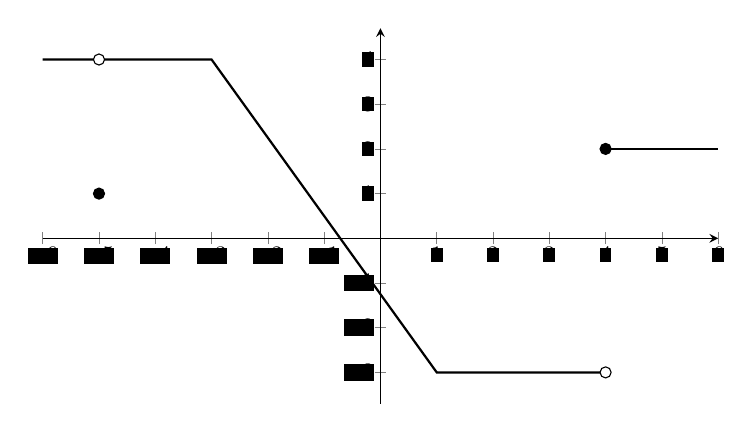
\begin{tikzpicture}
          \begin{axis}[cycle list=black, xtick={-6, -5, ..., 6}, ytick={-3, -2, ..., 4}, width=4in, height=2.5in]
            \addplot+[sharp plot] coordinates { (-6, 4) (-3, 4) (1, -3) (4, -3) };%
            \addplot+[sharp plot] coordinates { (4, 2) (6, 2) };%
            \addplot+[closed] coordinates { (-5, 1) (4, 2) };%
            \addplot+[open] coordinates { (-5, 4) (4, -3) };%
          \end{axis}
        \end{tikzpicture}
      \end{center}
    \end{solution}

  \item
    \begin{problem}[\vfill\newpage]
      $\displaystyle \lim_{x\to 1} g(x)= -3$.
    \end{problem}

    \begin{solution}
      Since $g(1) = -3$, this is exactly the statement that $g(x)$ is
      continuous at $x=1$.  Since $g(x)$ is continuous on $(-4, 4)$, this
      is \fbox{definitely true}.
    \end{solution}

  \item
    \begin{problem}[\vfill]
      $g$ has {\it at least} one $x$-intercept on $(-3, 1)$.
    \end{problem}

    \begin{solution}
      We know that the graph of $g$ includes $(-3, 4)$ and $(1, -3)$, and it's continuous between these two points. Any continuous graph that includes both these points must cross the $x$-axis, so this is \fbox{definitely true}. 
    \end{solution}

  \item
    \begin{problem}[\vfill]
      $g$ has {\it at least} one $x$-intercept on $(1, 5)$.
    \end{problem}

    \begin{solution}
      This is \fbox{not definitely true} since $g$ doesn't have to be continuous on all of $(1, 5)$, The graph in \ref{fall2012-ma-midterm1-3-II-a} is an example for which the statement is false. 
    \end{solution}

  \end{enumerate}

\item \label{fall2018-prefinal-practice3-3} \points{9} 

  In each part, decide whether there exists a polynomial with the specified properties.  If one exists, give the equation of an example and explain briefly how you know it has the specified properties.  If one does not exist, explain why.

  \begin{enumerate}

  \item
    \begin{problem}[\nstretch{1.75}]
      A polynomial $p(x)$ whose (only) intercepts are $(-1, 0)$, $(1, 0)$, $(2, 0)$, and $(0, 10)$, and which has $\displaystyle \lim_{x \to -\infty} p(x) = \lim_{x \to \infty} p(x)$.  
    \end{problem}

    \begin{solution}
      Since $\displaystyle \lim_{x \to -\infty} p(x) = \lim_{x \to \infty} p(x)$, the polynomial must have even degree. This polynomial has $x$-intercepts at $x = -1, 1, 2$, so it must have factors of $x + 1$, $x - 1$, and $x - 2$. To make a polynomial of even degree, we could raise one of these to the second power so that we end up with a degree 4 polynomial. So, we could have something like $f(x) = a(x + 1)^2 (x - 1)(x - 2)$. Now, we just need to pick an appropriate $a$ so that our example goes through $(0, 10)$: $f(0) = a (1)^2 (-1)(-2) = 2a$, so we want $a = 5$. Thus, \fbox{one example is ${f(x) = 5 (x + 1)^2 (x - 1)(x - 2)}$}.
    \end{solution}

  \item
    \begin{problem}[\vfill]
      A quadratic with a single inflection point at $x=1$.
    \end{problem}

    \begin{solution}
      This is \fbox{impossible}; a quadratic never changes concavity. (If the quadratic opens upward, it's always concave up; if it opens downward, it's always concave down.)
    \end{solution} 

  \item % added 2023

    \begin{problem}[\vfill\newpage]
      A polynomial $p(x)$ that has even degree but isn't an even function. 
    \end{problem}

    \begin{solution}
      \fbox{$p(x) = x (x - 1)$ is an example}; it has degree 2, but it isn't an even function because its roots (0 and 1) are not symmetric about the $y$-axis.
    \end{solution}

  \end{enumerate}

\item \label{optimization-box-cost-given-girth-volume} \points{14} 

  \begin{problem}[\newpage]
    A company is designing re-usable boxes for people to carry groceries in. The boxes will not have tops, to make it easier to load and unload groceries. They also decide that each box should have a volume of 360 in$^3$ and a ``girth'' (distance around) of 50 in. (The girth is the dotted line in the picture below.) The sides of the box will be made of a material that costs 2 cents per in$^2$; the bottom is to be made of a stronger material that costs 10 cents per in$^2$. Find the minimum cost of such a box. Be sure to justify your answer fully.

    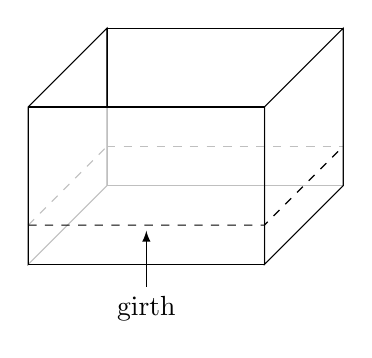
\begin{tikzpicture}
      \coordinate (O) at (0, 0); %
      \coordinate (W) at (3, 0); %
      \coordinate (L) at (1, 1); %
      \coordinate (H) at (0, 2); %
      \coordinate (girth) at (0, 0.5); %
      \begin{scope}[fill=white, fill opacity=0.75, draw=black, draw
        opacity=1]
        \filldraw ++(L) -- +(W) -- +($(W)+(H)$) -- +(H) -- cycle; %
        \draw[dashed] ++($(girth) + (L)$) -- +(W); %
        \filldraw (O) -- +(L) -- +($(L)+(H)$) -- +(H) -- cycle; %
        \draw[dashed] ++ (girth) -- +(L); %
        \filldraw ++(W) -- +(L) -- +($(L)+(H)$) -- +(H) -- cycle; %
        \filldraw (O) -- +(W) -- +($(W)+(H)$) -- +(H) -- cycle; %
        \draw[dashed] ++ (girth) -- ++(W) -- +(L); %
      \end{scope}
      \draw [yshift=4pt, ->] ($0.5*(W) - (0, 1em)$) node[below] {girth} --
      ($0.5*(W) + (girth)$); %
    \end{tikzpicture}
  \end{problem}

  \begin{solution}
    \highlight{Goal:} Minimize \goal{cost}.

    \highlight{Formula for goal:} The box is made up of 2 different types of material, so we can break the cost down as
    \begin{align}
      \text{cost} &= \text{cost of sides} + \text{cost of bottom} \nonumber \\
      &= (2 \text{ cents per in$^2$})(\text{area of sides}) + (10 \text{ cents per in$^2$})(\text{area of bottom}) \label{eq:optimization-box-cost-given-girth-volume}
    \end{align}
    At this point, it's convenient to \highlight{define some variables:}
    \begin{itemize}
    \item \goal{$C$} = cost
    \item $\ell$, $w$, $h$ = lengths shown in diagram below
    \end{itemize}
    \begin{center}
      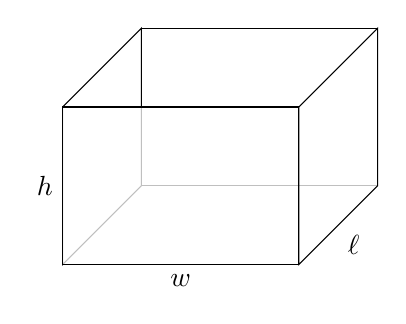
\begin{tikzpicture}
        \coordinate (O) at (0, 0); %
        \coordinate (W) at (3, 0); %
        \coordinate (L) at (1, 1); %
        \coordinate (H) at (0, 2); %
        \coordinate (girth) at (0, 0.5); %
        \begin{scope}[fill=white, fill opacity=0.75, draw=black, draw
          opacity=1]
          \filldraw ++(L) -- +(W) -- +($(W)+(H)$) -- +(H) -- cycle; %
          \filldraw (O) -- +(L) -- +($(L)+(H)$) -- +(H) -- cycle; %
          \filldraw ++(W) -- +(L) -- +($(L)+(H)$) -- +(H) -- cycle; %
          \filldraw (O) -- +(W) -- +($(W)+(H)$) -- +(H) -- cycle; %
        \end{scope}
        \draw ($0.5*(W)$) node[below]{$w$}; %
        \draw ($(W)+0.5*(L)$) node[anchor=north west]{$\ell$}; %
        \draw ($0.5*(H)$) node[left]{$h$}; %
      \end{tikzpicture}
    \end{center}
    Using these variables, we can rewrite (\ref{eq:optimization-box-cost-given-girth-volume}) as
    \begin{equation} \label{eq:optimization-box-cost-given-girth-volume-2}
      \goal{$C$} = 2 (2 w h + 2 \ell h) + 10 (w \ell)
    \end{equation}
    This formula involves $w, \ell, h$, so we need to \highlight{relate $w, \ell, h$ using something else we're told in the problem}:
    \begin{alignat*}{4}
      \text{volume} &= 360 & \hspace{1in} && \text{girth} &= 50 \\
      w \ell h &= 360 & & & 2w + 2\ell &= 50
    \end{alignat*}
    Rather than trying to solve for some of the variables in terms of the others, we can actually be a little more clever if we look at  (\ref{eq:optimization-box-cost-given-girth-volume-2}):
    \begin{align*}
      \goal{$C$} &= 2 h (2w + 2 \ell) + 10 w \ell \\
      &= 2 h (50) + 10 w \ell \\
      \intertext{In addition, we can use the equation $w \ell h = 360$ to write $w \ell = \frac{360}{h}$:}%
      &= 100h + 10 \cdot \frac{360}{h} \\
      \intertext{So, we have expressed $C$ as a function of just $h$:} %
      \goal{$C(h)$} &= 100 h + \frac{3600}{h}
    \end{align*}
    \highlight{Critical points:} $C'(h) = 100 - 3600 h^{-2} = 100 \left( 1 - \frac{36}{h^2} \right)$. This is undefined when $h = 0$, and it's 0 when $h = \pm 6$. Of course, we're only interested in positive values of $h$, so the only relevant critical point is $h = 6$.

    \highlight{Global minimum:} Let's use the Second Derivative Test: $C'(h) = 100 \left( 1 - 36 h^{-2} \right)$, so $C''(h) = 100 \cdot 72 h^{-3}$. Therefore, $C''(6) = \frac{7200}{6^3} > 0$. So, $h = 6$ is a local minimum; since it's the only critical point on $(0, \infty)$, it must be the global minimum on $(0, \infty)$.

    So, the minimum cost for such a box is $C(6) = 100 \left( 6 +
      \frac{36}{6} \right) = \boxed{1200 \text{ cents}}$.
  \end{solution}

\item \label{fall2018-final-practice1-9} \points{11} 

  The total waste in a country's landfills is a concern. An ongoing study is being conducted to predict the total waste levels in the future. Currently, there are 150,000,000 tons of waste in the country's landfills, and this amount is growing at an instantaneous rate of 2,000,000 tons per year.

  \begin{enumerate}
  \item
    \begin{problem}[\vfill]
      Suppose that the amount of waste continues to grow at a constant rate of 2,000,000 tons per year. Sketch a large graph modeling the amount of waste, in millions of tons, $t$ years from now. Call this $L(t).$
    \end{problem}

    \begin{solution}
      This graph is a line with $y$-intercept 150 and slope 2 million tons per year. 
      \begin{center}
        \answer{
          \begin{tikzpicture}
            \begin{axis}[ymin=0, ytick={150}, xlabel={$t$}, ylabel={waste (millions of tons)}]
              \addplot+[domain=0:75]{150+2*x} node[right] {$L(t)$};
            \end{axis}
          \end{tikzpicture}
        }
      \end{center}
    \end{solution}

  \item
    \begin{problem}
      Suppose instead that the amount of waste is modeled by an exponential function. On your graph from (a), sketch an exponential function that models the amount of waste, in millions of tons, $t$ years from now. Call this $E(t).$
    \end{problem}

    \begin{solution}
      Now, we want an exponential function with $y$-intercept 150, and the slope at $t = 0$ should be 2 million tons per year. That means the line from the previous part is a tangent line to $y = E(t)$ at $t = 0$:
      \begin{center}
        \answer{
          \begin{tikzpicture}
            \begin{axis}[ymin=0, ytick={150}, xlabel={$t$}, ylabel={waste (millions of tons)}, clip=false]
              \addplot+[domain=0:75]{150+2*x} node[right] {$L(t)$};
              \addplot+[domain=0:75, blue]{150*e^(x/75)} node[right] {$E(t)$};
            \end{axis}
          \end{tikzpicture}
        }
      \end{center}
    \end{solution}

  \item
    \begin{problem}[\vfill\newpage]
      Find a formula for $L(t).$
    \end{problem}

    \begin{solution}
      We know the slope and $y$-intercept, so we can write down the function directly: \fbox{$L(t) = 2t + 150$}. 
    \end{solution}

  \item
    \begin{problem}[\vfill]
      Since $E(t)$ is exponential, we can write $E(t) = C e^{kt}$. What are $C$ and $k$? 
    \end{problem}

    \begin{solution}
      Since $E(0) = 150$, we have $C e^0 = 150$, or \fbox{$C = 150$}.

      We also have $E'(0) = 2$. Since $E(t) = 150 e^{kt}$, we have
      \begin{align*}
        E'(t) &= 150 k e^{kt} \\
        E'(0) &= 150 k
      \end{align*}
      In order for this to equal $2$, we must have $\boxed{k = \dfrac{1}{75}}$. 
    \end{solution}

  \item
    \begin{problem}[\vfill\newpage]
      Which model predicts a higher amount of waste in the country's landfills one month from now? Explain briefly.
    \end{problem}

    \begin{solution}
      From the graphs we sketched, we can see that \answer{$E(t)$} always predicts a higher amount of waste than $L(t)$ (except at $t = 0$, where they're equal). 
    \end{solution}

  \end{enumerate}

\item \points{18}  

  In this problem, we'll look at $\displaystyle f(x) = \frac{x^2 - 4}{2x^2 + x - 10}$.

  \begin{enumerate}

  \item 
    \begin{problem}[\stretch{0.5}]
      Is $f(x)$ even, odd, or neither? Justify.
    \end{problem}

    \begin{solution}
      As always, we look at $f(-x)$:
      \[ f(-x) = \frac{(-x)^2 - 4}{2 (-x)^2 + (-x) - 10} = \frac{x^2 - 4}{2x^2 - x - 10}\]
      This isn't equal to $f(x)$, but it also isn't equal to $-f(x)$. So, $f$ is \fbox{neither even nor odd}.
    \end{solution}

  \item
    \begin{problem}[\vfill]
      Find all values of $x$ at which $f(x)$ is discontinuous. For each such value $a$, find $\displaystyle \lim_{x \to a} f(x)$. If $\displaystyle \lim_{x \to a} f(x)$ does not exist, find both $\displaystyle \lim_{x \to a^-} f(x)$ and $\displaystyle \lim_{x \to a^+} f(x)$. 
    \end{problem}

    \begin{solution}
      Since $f$ is given by a single non-piecewise formula, its discontinuities are where it's undefined. This happens when the denominator is equal to 0:
      \begin{align*}
        2x^2 + x - 10 &= 0 \\
        (2x + 5)(x - 2) &= 0 \\
        x &= -2.5, 2
      \end{align*}
      First, let's look at $\displaystyle \lim_{x \to -2.5} \frac{x^2 - 4}{2x^2 + x - 10}$. In this limit, the numerator tends to $2.5^2 - 4 > 0$ while the denominator tends to 0. So, we need to think about the sign of the denominator. When $x$ is just a bit bigger than $-2.5$ (like $x = -2.49$), the denominator $(2x + 5)(x - 2)$ is negative, so $\dfrac{x^2 - 4}{2x^2 + x - 10}$ will be very negative (since $x^2 - 4$ is positive). Therefore, $\displaystyle \boxed{\lim_{x \to -2.5^+} f(x) = -\infty}$.

      When $x$ is just a bit less than $-2.5$ (like $x = -2.51$), the denominator $(2x + 5)(x - 2)$ is positive, so $\dfrac{x^2 - 4}{2x^2 + x - 10}$ will be very positive. Therefore, $\displaystyle \boxed{\lim_{x \to -2.5^-} f(x) = \infty}$.

      Thus, \fbox{$\displaystyle \lim_{x \to -2.5} f(x)$ does not exist}.

      \begin{noanswer}
      Now, let's look at $\displaystyle \lim_{x \to 2} \frac{x^2 - 4}{2x^2 + x - 10}$. Here, the numerator and denominator both tend to 0, so we should try to factor and cancel something:
      \[ \frac{x^2 - 4}{2x^2 + x - 10} = \frac{(x - 2)(x + 2)}{(2x + 5)(x - 2)}.\]
      So, as long as $x \neq 2$, $\displaystyle f(x) = \frac{x + 2}{2x + 5}$. Therefore, $\boxed{\lim_{x \to 2} f(x) = \lim_{x \to 2} \frac{x + 2}{2x + 5} = \frac{4}{9}}$.
      \end{noanswer}
      \answeronly{$\displaystyle \lim_{x \to 2} f(x) = \frac{4}{9}$}
    \end{solution}

  \item
    \begin{problem}[\nstretch{0.25}]
      Find the $x$-intercepts of $f$.
    \end{problem}

    \begin{solution}
      We want to solve $f(x) = 0$, which happens when the numerator $(x-2)(x+2)$ is equal to 0. This happens when $x = \pm 2$, but $x = 2$ is not actually a root because we already saw that $f$ is undefined at $x = 2$. So, the only root is $\boxed{-2}$.
    \end{solution}

  \item 
    \begin{problem}[\vfill]
      Find all horizontal asymptotes of $f$, and justify your answer completely (and with correct notation). 
    \end{problem}

    \begin{solution}
      Finding the horizontal asymptotes of $f$ means calculating $\displaystyle \lim_{x \to \infty} f(x)$ and $\displaystyle \lim_{x \to -\infty} f(x)$. Let's first look at $\displaystyle \lim_{x \to \infty} f(x)$. In $\displaystyle \lim_{x \to \infty} \frac{x^2 - 4}{2x^2 + x - 10}$, both the numerator and denominator have a term that $\to \infty$. As we've seen, in a sum where some terms go to $\pm \infty$, we only need to keep the fastest-growing term. So,
      \[ \lim_{x \to \infty} \frac{x^2 - 4}{2x^2 + x - 10} = \lim_{x \to \infty} \frac{x^2}{2x^2} = \frac{1}{2}.\] Similarly,
      \[ \lim_{x \to -\infty} \frac{x^2 - 4}{2x^2 + x - 10} = \lim_{x \to -\infty} \frac{x^2}{2x^2} = \frac{1}{2}.\] So, $\boxed{y = \frac{1}{2}}$ is the only horizontal asymptote.
    \end{solution}

  \item
    \begin{problem}[\vfill\newpage]
      Use the information you've found in this problem to sketch a plausible graph of $f$. (We don't expect you to know the actual graph of $f$; we're just asking you to sketch something consistent with your answers to (a) - (d).) 
    \end{problem}

    \begin{solution}
      Here's the actual graph of $f$:
      \begin{center}
        \answer{
          \begin{tikzpicture}
            \begin{axis}[extra x ticks={-2.5}, ytick={-0.5}, xtick={-2, 2}, extra x tick style={grid style={dashed}}, enlarge y limits=false, width=5in]
              \addplot+[domain=-5:5, restrict y to domain=-2:2, samples=301] {(x+2)/(2*x+5)};%
              \addplot+[open] coordinates {(2, {4/9})}; %
              \addplot+[domain=-5:5, dashed] {0.5};%
            \end{axis}
          \end{tikzpicture}
        }
      \end{center}
    \end{solution}

    \begin{grading}
      We don't expect you to know the actual graph of $f$; rather, the graph you sketched should have the following features:
      \begin{itemize}
      \item $\displaystyle \lim_{x \to -2.5^-} f(x) = \infty$ and $\displaystyle \lim_{x \to -2.5^+} f(x) = -\infty$
      \item $\displaystyle \lim_{x \to -\infty} f(x) = \frac{1}{2}$ and $\displaystyle \lim_{x \to \infty} f(x) = \frac{1}{2}$
      \item The only root of $f(x)$ is at $x = -2$.
      \item $f$ has a removable discontinuity (hole) at $x = 2$.
      \end{itemize}
    \end{grading}

  \end{enumerate}

\item \label{fall2018-final-practice4-3} \points{9} 

  A train trip from Boston to Dover, New Hampshire is 68 miles long. 

  A train leaves from Boston for Dover at 5 am, traveling at a speed of 20 miles per hour. The train accelerates during the first 30 minutes of the trip, travels at a constant speed for 30 minutes, then decelerates for the next 20 minutes, arriving in Dover at 6:20 am. Let $s(t)$ be the position (in miles from Boston) of the train $t$ minutes after 5 am. (We will only consider the train's position between 5 am and 6:20 am, so the domain of $s(t)$ is $[0, 80]$.)

  \begin{enumerate} 
  \item \label{fall2018-final-practice4-3-tangent}

    \begin{problem}[\stretch{0.75}]
      Use a tangent line approximation to estimate the train's position (in miles from Boston) at 5:15 am.
    \end{problem}

    \begin{solution}
      When we find a tangent line to $y = f(x)$ at $x = a$, we're approximating $f$ by a function that increases at a \emph{constant} rate of $f'(a)$. How can we apply that here? 

      First, we have to start with a point we know, and the only point we know is $s(0) = 0$. We're told that $s'(0) = 20$ miles per hour. Using a tangent line approximation means supposing that the train continues traveling at a constant speed of 20 miles per hour; if this is the case, then between 5 and 5:15 am, the train would travel $(20 \text{ miles per hour}) \left( \dfrac{1}{4} \text{ hours} \right) = \boxed{5 \text{ miles}}$.

      \emph{Alternate method:} Graphically, we're using the tangent line to $y = s(t)$ at $t = 0$. Since the tangent line has slope 20 and includes the point $(0, 0)$, its equation is $y - 0 = 20 (t - 0)$, or $y = 20t$. This is a good approximation for $y = s(t)$ near $t = 0$, so
      \begin{align*}
        s(t) & \approx 20t \text{ for $t$ near 0} \\
        s(0.25) & \approx 20(0.25) = 5
      \end{align*}
    \end{solution}

  \item
    \begin{problem}[\stretch{0.3}]
      Is your approximation in \ref{fall2018-final-practice4-3-tangent} an overestimate or underestimate? Explain how you know.
    \end{problem}

    \begin{solution}
      To make our approximation, we assumed that the train was traveling at a constant speed of 20 miles per hour. But we know that the train was actually accelerating, so our estimate is an \fbox{underestimate}.

      \emph{Alternate method:} We can also approach this graphically. Since the train is accelerating on $(0, 30)$, the graph of $s(t)$ is concave up on $(0, 30)$. So, the tangent line at $t = 0$ will sit under the graph of $s(t)$.
    \end{solution}

  \item % added 2023

    \begin{problem}[\vfill\newpage]
      Is $s(t)$ invertible? If so, sketch a possible graph of $s^{-1}$, labeling any known points on the graph. If not, explain why not. 
    \end{problem}

    \begin{solution}
      Based on the description, $s(t)$ is increasing on its entire domain $[0, 80]$, so the graph of $s(t)$ will pass the horizontal line test. Therefore, $s(t)$ \fbox{is invertible}.

      To sketch a graph of $s^{-1}$, it's helpful to first sketch a graph of $s$, since then we can just flip that over the line $y = x$ (or really, $s = t$).

      Based on the given information, the graph of $s(t)$ is concave up on $(0, 30)$, linear on $(30, 60)$, and concave down on $(60, 80)$. So, here's a possible graph of $s(t)$ (we've colored the 3 ``pieces'' of the graph in different colors just to make them more clear):
      \begin{center}
        \begin{tikzpicture}
          \begin{axis}[xtick={30, 60, 80}, ytick={68}, enlarge x limits=auto, axis equal image, clip=false]; %
            \addplot+[domain=0:30, hotpink] {68/3500*x^2}; %
            \addplot+[domain=30:60, green!90!black] {68/3500*(60*(x-30)+30^2)}; %
            \addplot+[domain=60:80, skyblue] {68/3500*(3600-(x-90)^2)}; %
            \addplot+[closed] coordinates {(80, 68)} node[right]{$(80, 68)$}; % 
          \end{axis}
        \end{tikzpicture}
      \end{center}
      So, here's a possible graph of $s^{-1}$:
      \begin{center}
        \answer{
          \begin{tikzpicture}
            \begin{axis}[ytick={30, 60, 80}, xtick={68}, enlarge x limits=auto, axis equal image, clip=false]; %
              \begin{scope}[black!40!white, dashed]
                \addplot+[domain=0:30] {68/3500*x^2}; %
                \addplot+[domain=30:60] {68/3500*(60*(x-30)+30^2)}; %
                \addplot+[domain=60:80] {68/3500*(3600-(x-90)^2)} node[right]{$s$}; %
              \end{scope}
              \addplot+[domain=0:30] (68/3500*x^2, x); %
              \addplot+[domain=30:60] (68/3500*(60*(x-30)+30^2), x); %
              \addplot+[domain=60:80] (68/3500*(3600-(x-90)^2), x) node[above]{$s^{-1}$}; %
              \addplot+[closed] coordinates {(68, 80)} node[right]{$(68, 80)$}; % 
            \end{axis}
          \end{tikzpicture}
        }
      \end{center}
    \end{solution}

    \begin{grading}
      The key features your graph should have are:
      \begin{itemize}
      \item The domain is $[0, 68]$, and the range is $[0, 80]$.
      \item $s^{-1}$ is increasing everywhere.
      \item $s^{-1}$ is concave down until it reaches a height of 30, linear between a height of 30 and 60, and concave up when the height is $> 60$. 
      \end{itemize}
    \end{grading}

  \end{enumerate} 

\item \label{fall2018-prefinal-practice2-7-shortened} \points{6} 

  \begin{problem}
    Let $f(x)=2x^5+5x^4-10x^3+1$. Does $f(x)$ attain a global maximum on $[-1, 2]$? If so, give the maximum value and where it occurs. If not, explain why not.

    What about a global minimum? 
  \end{problem}

  \begin{solution}
    Since $f$ is continuous and $[-1, 2]$ is a closed interval, the Extreme Value Theorem guarantees that $f$ attains both a global minimum and a global maximum on $[-1, 2]$. To find them, we need to look at critical points and the endpoints $-1, 2$ of the domain.

    First, let's find critical points. 
    \begin{align*}
      f'(x)&=10x^4+20x^3-30x^2 \\
      &=10x^2(x^2+2x-3) \\
      &=10x^2(x+3)(x-1)
    \end{align*}
    This is never undefined, and it's 0 when $x=-3, 0, 1$. Since we're interested in the interval $[-1, 2]$, we can ignore $x = -3$.

    Now, we just plug the critical points and endpoints into $f$ to see which gives us the highest value:
    \begin{itemize}[nosep]
    \item $f(-1)=14$
    \item $f(0)=1$
    \item $f(1)=-2$
    \item $f(2)=65$
    \end{itemize}
    So, on $[-1, 2]$, $f$ has a \fbox{global maximum value of 65 at $x = 2$ and a global minimum value of $-2$ at $x = 1$}.
  \end{solution}

  \pspace{\newpage}

\item 
  \label{fall2012-ma-prefinal-1-modified} \points{12} 
\finishexam

  A company is producing tablet computers. The tablets cost \$250 each to produce. Their market research suggests:

  \begin{itemize}[nosep]    
  \item If they price the tablets at \$300 each, they will sell 12,000 units in the first month.
  \item For each \$10 increase above \$300, the number of tablets they will sell will decrease by 5\%.
  \end{itemize}

  \begin{enumerate}

  \item
    \begin{problem}[\vfill]
      Let $N(x)$ be the number of tablets that they will sell in the first
      month if they price their tablet $x$ dollars {\it above \$300}.
      Find a formula for $N(x)$.
    \end{problem}

    \begin{solution}
      Let's make a table. When the price of the tablets is \$300 (so $x = 0$), they will sell 12,000 tablets. For each \$10 increase in $x$, the number of tablets sold is multiplied by $0.95$. So, we get the following table:
      \begin{center}
        \begin{tabular}{r | l}
          $x$ & $N(x)$ \\
          \hline
          $0$ & $12000$ \\
          $10$ & $12000 (0.95)$ \\
          $20$ & $12000 (0.95)^2$ \\
          $30$ & $12000 (0.95)^3$ \\
          $\mathrel{\makebox[\widthof{30}]{\vdots}}$ &
          $\mathrel{\makebox[\widthof{12000}]{\vdots}}$
        \end{tabular}
      \end{center}
      From the table, we can see that the pattern is $\boxed{N(x) = 12000 (0.95)^{x/10}}$.
    \end{solution}

  \item
    \begin{problem}[\vfill\newpage]
      If the company wants to sell $10,000$ tablets in the first month, 
      what should they set the price of the tablets to be?
    \end{problem}

    \begin{solution} 
      Since $N(x)$ gives the number of tablets sold, we want to solve for when $N(x) = 10,000$:
      \begin{align*}
        12,000 (0.95)^{x/10} &= 10,000 \\
        (0.95)^{x/10} &= \frac{10,000}{12,000} = \frac{5}{6} \\
        \intertext{Taking $\log_{0.95}$ of both sides,}
        \frac{x}{10} &= \log_{0.95} \left( \frac{5}{6} \right) \\
        x &= 10 \log_{0.95} \left( \frac{5}{6} \right)         
      \end{align*}
      Finally, we should remember that $x$ doesn't represent the price itself, but rather the number of dollars over \$300, so the price of the tablets should be $\boxed{300 + 10 \log_{0.95} \left( \frac{5}{6} \right) \text{ dollars}}$. (This is about \$335.54.)
    \end{solution}

  \item

    \begin{problem}[\stretch{0.75}]
      Find a formula for $P(x)$, the company's total profit in the first
      month if they price their tablets at $x$ dollars above \$300.
    \end{problem}

    \begin{solution}
      \highlight{Goal:} Express \goal{profit} as a function of $x$.      
      \begin{align*}
        \goal{\text{profit}} &= \text{revenue} - \text{cost} \\
        &= (\text{number of tablets})(\text{price per tablet}) -
        (\text{number of tablets}) (\text{cost per tablet}) \\
        \intertext{We want to express all of these quantities in terms of $x$. If the company prices the tablets at $x$ dollars above \$300, then the number they will sell is exactly $N(x)$, so we can rewrite the above expression as}%
        &= N(x) (x+300) - N(x) (250)\\
        &=  N(x) (x + 50) \\
        & = \boxed{12,000(.95)^{x/10} (x + 50)}
      \end{align*}
    \end{solution}

  \item
    \begin{problem}[\stretch{0.5}]
      It turns out that $P'(200)$ is negative (you do not need to verify this). Interpret in words what this says about profits.
    \end{problem}

    \begin{solution}
      \answer{When the price is set at \$200 above \$300 (i.e., when the tablets cost \$500 each), a small increase in price will lead to a decrease in profit.}
    \end{solution}

  \end{enumerate}

\end{enumerate}

\end{document}
